% Options for packages loaded elsewhere
\PassOptionsToPackage{unicode}{hyperref}
\PassOptionsToPackage{hyphens}{url}
%
\documentclass[
  a4paper,
]{book}

\usepackage{amsmath,amssymb}
\usepackage{iftex}
\ifPDFTeX
  \usepackage[T1]{fontenc}
  \usepackage[utf8]{inputenc}
  \usepackage{textcomp} % provide euro and other symbols
\else % if luatex or xetex
  \usepackage{unicode-math}
  \defaultfontfeatures{Scale=MatchLowercase}
  \defaultfontfeatures[\rmfamily]{Ligatures=TeX,Scale=1}
\fi
\usepackage{lmodern}
\ifPDFTeX\else  
    % xetex/luatex font selection
  \setmainfont[]{NanumBarunGothic.otf}
  \setsansfont[]{NanumBarunGothic.otf}
  \setmonofont[]{NanumBarunGothic.otf}
\fi
% Use upquote if available, for straight quotes in verbatim environments
\IfFileExists{upquote.sty}{\usepackage{upquote}}{}
\IfFileExists{microtype.sty}{% use microtype if available
  \usepackage[]{microtype}
  \UseMicrotypeSet[protrusion]{basicmath} % disable protrusion for tt fonts
}{}
\makeatletter
\@ifundefined{KOMAClassName}{% if non-KOMA class
  \IfFileExists{parskip.sty}{%
    \usepackage{parskip}
  }{% else
    \setlength{\parindent}{0pt}
    \setlength{\parskip}{6pt plus 2pt minus 1pt}}
}{% if KOMA class
  \KOMAoptions{parskip=half}}
\makeatother
\usepackage{xcolor}
\usepackage[tmargin=2cm,bmargin=2cm,lmargin=2cm,rmargin=2cm]{geometry}
\setlength{\emergencystretch}{3em} % prevent overfull lines
\setcounter{secnumdepth}{5}
% Make \paragraph and \subparagraph free-standing
\ifx\paragraph\undefined\else
  \let\oldparagraph\paragraph
  \renewcommand{\paragraph}[1]{\oldparagraph{#1}\mbox{}}
\fi
\ifx\subparagraph\undefined\else
  \let\oldsubparagraph\subparagraph
  \renewcommand{\subparagraph}[1]{\oldsubparagraph{#1}\mbox{}}
\fi

\usepackage{color}
\usepackage{fancyvrb}
\newcommand{\VerbBar}{|}
\newcommand{\VERB}{\Verb[commandchars=\\\{\}]}
\DefineVerbatimEnvironment{Highlighting}{Verbatim}{commandchars=\\\{\}}
% Add ',fontsize=\small' for more characters per line
\usepackage{framed}
\definecolor{shadecolor}{RGB}{241,243,245}
\newenvironment{Shaded}{\begin{snugshade}}{\end{snugshade}}
\newcommand{\AlertTok}[1]{\textcolor[rgb]{0.68,0.00,0.00}{#1}}
\newcommand{\AnnotationTok}[1]{\textcolor[rgb]{0.37,0.37,0.37}{#1}}
\newcommand{\AttributeTok}[1]{\textcolor[rgb]{0.40,0.45,0.13}{#1}}
\newcommand{\BaseNTok}[1]{\textcolor[rgb]{0.68,0.00,0.00}{#1}}
\newcommand{\BuiltInTok}[1]{\textcolor[rgb]{0.00,0.23,0.31}{#1}}
\newcommand{\CharTok}[1]{\textcolor[rgb]{0.13,0.47,0.30}{#1}}
\newcommand{\CommentTok}[1]{\textcolor[rgb]{0.37,0.37,0.37}{#1}}
\newcommand{\CommentVarTok}[1]{\textcolor[rgb]{0.37,0.37,0.37}{\textit{#1}}}
\newcommand{\ConstantTok}[1]{\textcolor[rgb]{0.56,0.35,0.01}{#1}}
\newcommand{\ControlFlowTok}[1]{\textcolor[rgb]{0.00,0.23,0.31}{#1}}
\newcommand{\DataTypeTok}[1]{\textcolor[rgb]{0.68,0.00,0.00}{#1}}
\newcommand{\DecValTok}[1]{\textcolor[rgb]{0.68,0.00,0.00}{#1}}
\newcommand{\DocumentationTok}[1]{\textcolor[rgb]{0.37,0.37,0.37}{\textit{#1}}}
\newcommand{\ErrorTok}[1]{\textcolor[rgb]{0.68,0.00,0.00}{#1}}
\newcommand{\ExtensionTok}[1]{\textcolor[rgb]{0.00,0.23,0.31}{#1}}
\newcommand{\FloatTok}[1]{\textcolor[rgb]{0.68,0.00,0.00}{#1}}
\newcommand{\FunctionTok}[1]{\textcolor[rgb]{0.28,0.35,0.67}{#1}}
\newcommand{\ImportTok}[1]{\textcolor[rgb]{0.00,0.46,0.62}{#1}}
\newcommand{\InformationTok}[1]{\textcolor[rgb]{0.37,0.37,0.37}{#1}}
\newcommand{\KeywordTok}[1]{\textcolor[rgb]{0.00,0.23,0.31}{#1}}
\newcommand{\NormalTok}[1]{\textcolor[rgb]{0.00,0.23,0.31}{#1}}
\newcommand{\OperatorTok}[1]{\textcolor[rgb]{0.37,0.37,0.37}{#1}}
\newcommand{\OtherTok}[1]{\textcolor[rgb]{0.00,0.23,0.31}{#1}}
\newcommand{\PreprocessorTok}[1]{\textcolor[rgb]{0.68,0.00,0.00}{#1}}
\newcommand{\RegionMarkerTok}[1]{\textcolor[rgb]{0.00,0.23,0.31}{#1}}
\newcommand{\SpecialCharTok}[1]{\textcolor[rgb]{0.37,0.37,0.37}{#1}}
\newcommand{\SpecialStringTok}[1]{\textcolor[rgb]{0.13,0.47,0.30}{#1}}
\newcommand{\StringTok}[1]{\textcolor[rgb]{0.13,0.47,0.30}{#1}}
\newcommand{\VariableTok}[1]{\textcolor[rgb]{0.07,0.07,0.07}{#1}}
\newcommand{\VerbatimStringTok}[1]{\textcolor[rgb]{0.13,0.47,0.30}{#1}}
\newcommand{\WarningTok}[1]{\textcolor[rgb]{0.37,0.37,0.37}{\textit{#1}}}

\providecommand{\tightlist}{%
  \setlength{\itemsep}{0pt}\setlength{\parskip}{0pt}}\usepackage{longtable,booktabs,array}
\usepackage{calc} % for calculating minipage widths
% Correct order of tables after \paragraph or \subparagraph
\usepackage{etoolbox}
\makeatletter
\patchcmd\longtable{\par}{\if@noskipsec\mbox{}\fi\par}{}{}
\makeatother
% Allow footnotes in longtable head/foot
\IfFileExists{footnotehyper.sty}{\usepackage{footnotehyper}}{\usepackage{footnote}}
\makesavenoteenv{longtable}
\usepackage{graphicx}
\makeatletter
\def\maxwidth{\ifdim\Gin@nat@width>\linewidth\linewidth\else\Gin@nat@width\fi}
\def\maxheight{\ifdim\Gin@nat@height>\textheight\textheight\else\Gin@nat@height\fi}
\makeatother
% Scale images if necessary, so that they will not overflow the page
% margins by default, and it is still possible to overwrite the defaults
% using explicit options in \includegraphics[width, height, ...]{}
\setkeys{Gin}{width=\maxwidth,height=\maxheight,keepaspectratio}
% Set default figure placement to htbp
\makeatletter
\def\fps@figure{htbp}
\makeatother

\usepackage{kotex}
\makeatletter
\makeatother
\makeatletter
\@ifpackageloaded{bookmark}{}{\usepackage{bookmark}}
\makeatother
\makeatletter
\@ifpackageloaded{caption}{}{\usepackage{caption}}
\AtBeginDocument{%
\ifdefined\contentsname
  \renewcommand*\contentsname{Table of contents}
\else
  \newcommand\contentsname{Table of contents}
\fi
\ifdefined\listfigurename
  \renewcommand*\listfigurename{List of Figures}
\else
  \newcommand\listfigurename{List of Figures}
\fi
\ifdefined\listtablename
  \renewcommand*\listtablename{List of Tables}
\else
  \newcommand\listtablename{List of Tables}
\fi
\ifdefined\figurename
  \renewcommand*\figurename{Figure}
\else
  \newcommand\figurename{Figure}
\fi
\ifdefined\tablename
  \renewcommand*\tablename{Table}
\else
  \newcommand\tablename{Table}
\fi
}
\@ifpackageloaded{float}{}{\usepackage{float}}
\floatstyle{ruled}
\@ifundefined{c@chapter}{\newfloat{codelisting}{h}{lop}}{\newfloat{codelisting}{h}{lop}[chapter]}
\floatname{codelisting}{Listing}
\newcommand*\listoflistings{\listof{codelisting}{List of Listings}}
\makeatother
\makeatletter
\@ifpackageloaded{caption}{}{\usepackage{caption}}
\@ifpackageloaded{subcaption}{}{\usepackage{subcaption}}
\makeatother
\makeatletter
\@ifpackageloaded{tcolorbox}{}{\usepackage[skins,breakable]{tcolorbox}}
\makeatother
\makeatletter
\@ifundefined{shadecolor}{\definecolor{shadecolor}{rgb}{.97, .97, .97}}
\makeatother
\makeatletter
\makeatother
\makeatletter
\makeatother
\ifLuaTeX
  \usepackage{selnolig}  % disable illegal ligatures
\fi
\IfFileExists{bookmark.sty}{\usepackage{bookmark}}{\usepackage{hyperref}}
\IfFileExists{xurl.sty}{\usepackage{xurl}}{} % add URL line breaks if available
\urlstyle{same} % disable monospaced font for URLs
\hypersetup{
  pdftitle={R Programming for Engineering Biology},
  hidelinks,
  pdfcreator={LaTeX via pandoc}}

\title{R Programming for Engineering Biology}
\author{}
\date{}

\begin{document}
\frontmatter
\maketitle
\ifdefined\Shaded\renewenvironment{Shaded}{\begin{tcolorbox}[borderline west={3pt}{0pt}{shadecolor}, interior hidden, sharp corners, enhanced, breakable, boxrule=0pt, frame hidden]}{\end{tcolorbox}}\fi

\renewcommand*\contentsname{Table of contents}
{
\setcounter{tocdepth}{2}
\tableofcontents
}
\mainmatter
\bookmarksetup{startatroot}

\hypertarget{course-introduction}{%
\chapter{Course introduction}\label{course-introduction}}

\hypertarget{uxc18cuxac1c}{%
\section{소개}\label{uxc18cuxac1c}}

카이스트 공학생물학 대학원 강의용 강의노트 (2023.11)

\hypertarget{uxbaa9uxcc28}{%
\section{목차}\label{uxbaa9uxcc28}}

\begin{itemize}
\tightlist
\item
  \protect\hyperlink{introduction}{Chapter 1: Introduction}
\item
  \protect\hyperlink{quarto-and-markdown}{Chapter 2: Quarto and
  Markdown}
\end{itemize}

\hypertarget{uxb370uxc774uxd130-uxbd84uxc11d}{%
\section{데이터 분석}\label{uxb370uxc774uxd130-uxbd84uxc11d}}

\begin{figure}

{\centering 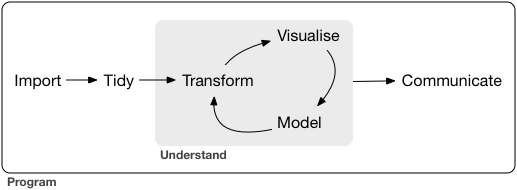
\includegraphics[width=5.66667in,height=\textheight]{images/07/data-science.png}

}

\caption{from https://r4ds.had.co.nz/}

\end{figure}

posit의 대표적 개발자인 해들리위컴은 \texttt{R\ for\ Data\ Science}의
서두에 위와 같은 그림으로 데이터과학을 설명하고 있습니다. 원본 데이터는
Tidy 형태로 R로 불러와야 하고 언제든 분석에 맞는 형태로 \texttt{변형} 할
수 있어야 합니다. 그리고 항상 \texttt{시각화}를 통해 데이터를 직접
검증해야하고 \texttt{모델}을 사용해서 원하는 분석을 수행합니다. 분석
후에는 \texttt{공유}를 통해 객관적인 검증이 필요합니다. R은 이 모든
과정을 빠르고 효율적으로 수행할 수 있는 최고의 언어입니다. 데이터과학
입장에서는 위 도구들을 둘러싸고 있는것이 \texttt{프로그래밍} 입니다.

\hypertarget{uxb77cuxc774uxc120uxc2a4}{%
\section{라이선스}\label{uxb77cuxc774uxc120uxc2a4}}

이 책은 Creative Commons Attribution-NonCommercial 4.0 International (CC
BY-NC 4.0) 라이선스에 따라 제공됩니다.

\bookmarksetup{startatroot}

\hypertarget{introduction}{%
\chapter{Introduction}\label{introduction}}

\hypertarget{r-rstudio-introduction}{%
\section{R / RStudio Introduction}\label{r-rstudio-introduction}}

R은 통계학, 생물통계학, 유전학 등의 연구 분야에서 널리 사용되는 오픈소스
프로그래밍 언어입니다. S 언어에서 파생되었고, 데이터 분석 및 가시화
패키지들이 강점입니다. 최근 인공지능의 관심이 크게 증가하면서 python
언어의 수요가 더 증가하긴 했으나 특히 중,소규모의 데이터 전처리와
가시화, 통계분석 측면에서 여전히 많은 사용자를 확보하고 있는 언어입니다.

R언어가 주목을 받고 두터운 사용자 층을 확보할 수 있게된 핵심 동력이
Rstudio 입니다. Rstudio를 개발한 Posit은 자체적으로 최고수준의 오픈소스
개발팀이 있으며 tidyverse, tidymodel, shiny 등의 데이터 분석 및 가시화
관련 주요 패키지를 개발하였고 정기적으로 conference 개최를 하면서 기술
보급의 핵심 역할을 하고 있습니다. R을 활용한 데이터 분석은 tidyverse 가
나오기 이전과 이후로 분리될 수 있을 정도로 tidyverse는 많은 변화와
효율향상을 이뤄냈습니다.

\hypertarget{installing-r-rstudio}{%
\section{Installing R / RStudio}\label{installing-r-rstudio}}

R 사용을 위해서는 R 언어의 코어 프로그램을 먼저 설치하고 그 다음 R
언어용 IDE(Integrated Development Environment)인 RStudio 설치가
필요합니다. Rstudio는 R 언어를 위한 오픈소스 기반 통합개발환경(IDE)으로
R 프로그래밍을 위한 편리한 기능들을 제공해 줍니다.

\hypertarget{installing-r}{%
\subsection{Installing R}\label{installing-r}}

\begin{itemize}
\tightlist
\item
  R 공식 웹사이트 {[}https://www.r-project.org/{]}를 방문하세요. 왼쪽
  메뉴 상단에 위치한 CRAN을 클릭합니다.
\item
  목록에서 한국 미러 사이트 중 하나를 선택합니다.
\item
  `Windows용 R 다운로드'를 클릭한 다음 'base' 링크로 들어갑니다.
\item
  'Windows용 R x.x.x 다운로드'를 클릭하여 실행 가능한 프로그램을
  다운로드합니다.
\item
  다운로드된 R-x.x.x-win.exe 파일을 로컬 컴퓨터에서 실행합니다 (2023년
  11월 현재, R의 최신 버전은 4.3.2입니다).
\item
  설치 프로그램의 지시에 따라 R 언어 소프트웨어 설치를 완료합니다.
\end{itemize}

\hypertarget{installing-rstudio}{%
\subsection{Installing RStudio}\label{installing-rstudio}}

\begin{itemize}
\tightlist
\item
  Posit의 Rstudio 공식 {[}https://posit.co/{]} 웹사이트를 방문한 다음,
  페이지 상단의 'Products \textgreater{} RStudio IDE'를 클릭합니다.
\item
  `Open Source Edition' Free의 'Download Rstudio Desktop'을 클릭합니다.
\item
  'Download Rstudio'의 'Download Rstudio desktop for windows'를 클릭하여
  다운로드를 시작합니다.
\item
  다운로드된 RStudio-x.x.x.exe 파일을 로컬 컴퓨터에서 실행합니다 (2023년
  11월 현재, RStudio 데스크톱의 최신 버전은 2023.09입니다).
\item
  설치 가이드를 따라 설치를 완료합니다.
\end{itemize}

\hypertarget{posit-cloud}{%
\subsection{Posit Cloud}\label{posit-cloud}}

Posit Cloud는 클라우드에서 RStudio를 제공하여 사용자가 설치 및 설정 없이
브라우저에서 직접 RStudio를 사용할 수 있게 합니다.

\begin{itemize}
\tightlist
\item
  posit.cloud에 방문하여 사용자로 등록합니다 (Google 계정을 사용할 수
  있습니다).
\item
  로그인하고 'Cloud Free'를 선택하여 시작합니다.
\item
  이 환경에서는 1GB의 RAM과 1 CPU를 무료로 제공합니다.
\end{itemize}

\hypertarget{rstudio-interface-and-keyboard-shortcuts}{%
\section{RStudio Interface and Keyboard
Shortcuts}\label{rstudio-interface-and-keyboard-shortcuts}}

RStudio는 코드 편집 창, 콘솔 창, 환경 및 파일 패널을 제공합니다.

\textbf{주요 키보드 단축키}

\begin{itemize}
\tightlist
\item
  코드 실행: \texttt{Ctrl} + \texttt{Enter}
\item
  콘솔 창으로 이동: \texttt{Ctrl} + \texttt{2}
\item
  코드 편집 창으로 이동: \texttt{Ctrl} + \texttt{1}
\item
  저장: \texttt{Ctrl} + \texttt{S}
\item
  코드 주석 처리: \texttt{Ctrl} + \texttt{Shift} + \texttt{C}
\end{itemize}

\hypertarget{starting-a-project}{%
\section{Starting a Project}\label{starting-a-project}}

'RStudio'에서 '파일 \textgreater{} 새 프로젝트'로 가서 새 프로젝트를
시작할 수 있습니다.

\begin{itemize}
\tightlist
\item
  Hello World Example
\item
  Create a new R file and execute the following code:
\end{itemize}

\begin{Shaded}
\begin{Highlighting}[]
\NormalTok{mystring }\OtherTok{\textless{}{-}} \StringTok{"Hello }\SpecialCharTok{\textbackslash{}n}\StringTok{ world!"}
\FunctionTok{cat}\NormalTok{(mystring)}
\FunctionTok{print}\NormalTok{(mystring)}
\end{Highlighting}
\end{Shaded}

\hypertarget{getting-help}{%
\section{Getting Help}\label{getting-help}}

R은 방대한 도움말 데이터를 제공하며, 다음과 같은 명령어로 특정 함수의
도움말과 예제를 찾아볼 수 있습니다.

\begin{Shaded}
\begin{Highlighting}[]
\FunctionTok{help}\NormalTok{(}\StringTok{"mean"}\NormalTok{)}
\NormalTok{?mean}
\FunctionTok{example}\NormalTok{(}\StringTok{"mean"}\NormalTok{)}
\FunctionTok{help.search}\NormalTok{(}\StringTok{"mean"}\NormalTok{)}
\NormalTok{??mean}
\FunctionTok{help}\NormalTok{(}\AttributeTok{package=}\StringTok{"MASS"}\NormalTok{)}
\end{Highlighting}
\end{Shaded}

RStudio 치트시트는 다양한 R 기능을 한눈에 알아볼 수 있게 만든 cheatsheet
형태의 문서를 참고할 수 있습니다. 자세한 내용은
\href{https://posit.co/resources/cheatsheets/}{Posit Cheatsheets}를
참조하세요.

\hypertarget{r-uxd328uxd0a4uxc9c0uxc640-uxb370uxc774uxd130uxc14b}{%
\section{R 패키지와
데이터셋}\label{r-uxd328uxd0a4uxc9c0uxc640-uxb370uxc774uxd130uxc14b}}

R 패키지는 함수와 데이터셋의 묶음으로, 다른 사람들이 만들어 놓은 코드나
기능을 가져와 사용함으로써 코드 작성의 수고로움을 줄이고, 편리하고
검증된 함수(기능)를 빠르게 도입하여 사용할 수 있습니다. 예를 들어
\texttt{sd()} 함수는 \texttt{stats} 패키지에서 제공하는 함수로, 표준편차
계산을 위한 별도의 함수를 만들어서 사용할 필요가 없습니다.

\begin{Shaded}
\begin{Highlighting}[]
\FunctionTok{library}\NormalTok{(UsingR)}
\end{Highlighting}
\end{Shaded}

\hypertarget{uxd328uxd0a4uxc9c0-uxc124uxce58-uxbc0f-uxb85cuxb4dc}{%
\subsection{패키지 설치 및
로드}\label{uxd328uxd0a4uxc9c0-uxc124uxce58-uxbc0f-uxb85cuxb4dc}}

패키지는 CRAN 또는 Bioconductor와 같은 저장소에서 구할 수 있으며, 아래와
같이 RStudio를 이용하거나 콘솔창에서 \texttt{install.packages()} 함수를
이용할 수 있습니다.

\begin{Shaded}
\begin{Highlighting}[]
\FunctionTok{install.packages}\NormalTok{(}\StringTok{"UsingR"}\NormalTok{)}
\end{Highlighting}
\end{Shaded}

\hypertarget{uxc124uxce58-uxb514uxb809uxd1a0uxb9ac-uxd655uxc778uxd558uxae30}{%
\subsection{설치 디렉토리
확인하기}\label{uxc124uxce58-uxb514uxb809uxd1a0uxb9ac-uxd655uxc778uxd558uxae30}}

R 및 패키지의 설치 디렉토리는 다음 명령어로 확인할 수 있습니다.

\begin{Shaded}
\begin{Highlighting}[]
\FunctionTok{.libPaths}\NormalTok{()}
\FunctionTok{path.package}\NormalTok{()}
\end{Highlighting}
\end{Shaded}

\hypertarget{uxd328uxd0a4uxc9c0-uxb370uxc774uxd130-uxc0acuxc6a9uxd558uxae30}{%
\subsection{패키지 데이터
사용하기}\label{uxd328uxd0a4uxc9c0-uxb370uxc774uxd130-uxc0acuxc6a9uxd558uxae30}}

패키지 안에 포함된 데이터도 사용할 수 있으며 \texttt{data()} 함수를
이용해서 패키지 데이터를 사용자 작업공간에 복사해서 사용할 수 있습니다.

\begin{Shaded}
\begin{Highlighting}[]
\FunctionTok{data}\NormalTok{(rivers)}
\FunctionTok{length}\NormalTok{(rivers)}
\FunctionTok{class}\NormalTok{(rivers)}
\FunctionTok{data}\NormalTok{(}\AttributeTok{package=}\StringTok{"UsingR"}\NormalTok{)}
\FunctionTok{library}\NormalTok{(HistData)}
\FunctionTok{head}\NormalTok{(Cavendish)}
\FunctionTok{str}\NormalTok{(Cavendish)}
\end{Highlighting}
\end{Shaded}

\begin{center}\rule{0.5\linewidth}{0.5pt}\end{center}

이 저작물은 크리에이티브 커먼즈 저작자표시-비영리-변경금지 4.0 국제
라이선스에 따라 이용할 수 있습니다.

\bookmarksetup{startatroot}

\hypertarget{quarto-and-markdown}{%
\chapter{Quarto and Markdown}\label{quarto-and-markdown}}

\hypertarget{introduction-1}{%
\section{Introduction}\label{introduction-1}}

Quarto는 데이터 과학에서 사용되는 코드와 리포트를 결합할 수 있는 통합
문서 시스템입니다. 마이크로소프트 워드나 한글과 같은 워드 프로세서에서
프로그래밍 코드와 데이터 분석을 수행할 수 있는 것처럼, Quarto를 사용하면
텍스트 기반의 마크다운 문법으로 문서를 작성하고 다양한 형식의 출력물로
변환할 수 있습니다. 이러한 출력물에는 HTML, PDF, Word 문서, 슬라이드 쇼,
책, 웹사이트 등이 포함됩니다.

Quarto에 대한 더 자세한 정보는 Quarto 공식 웹사이트에서 확인할 수
있습니다. 해당 웹사이트에는 Quarto 소개 동영상과
\href{https://quarto.org/docs/}{Quarto 공식 사이트 메뉴얼}이 있으며,
Quarto를 사용할 때 참고할 수 있는
\href{https://quarto.org/docs/cheatsheets/quarto}{cheatsheet}도
제공됩니다.

\hypertarget{quartouxc758-uxae30uxbcf8-uxc791uxb3d9-uxc6d0uxb9ac}{%
\section{Quarto의 기본 작동
원리}\label{quartouxc758-uxae30uxbcf8-uxc791uxb3d9-uxc6d0uxb9ac}}

Quarto는 plain text 기반으로 작성되며 \texttt{.qmd} 라는 확장자를 갖는
파일로 저장됩니다. 다음과 같은 텍스트 파일이 Quarto 파일의 전형적인
예입니다.

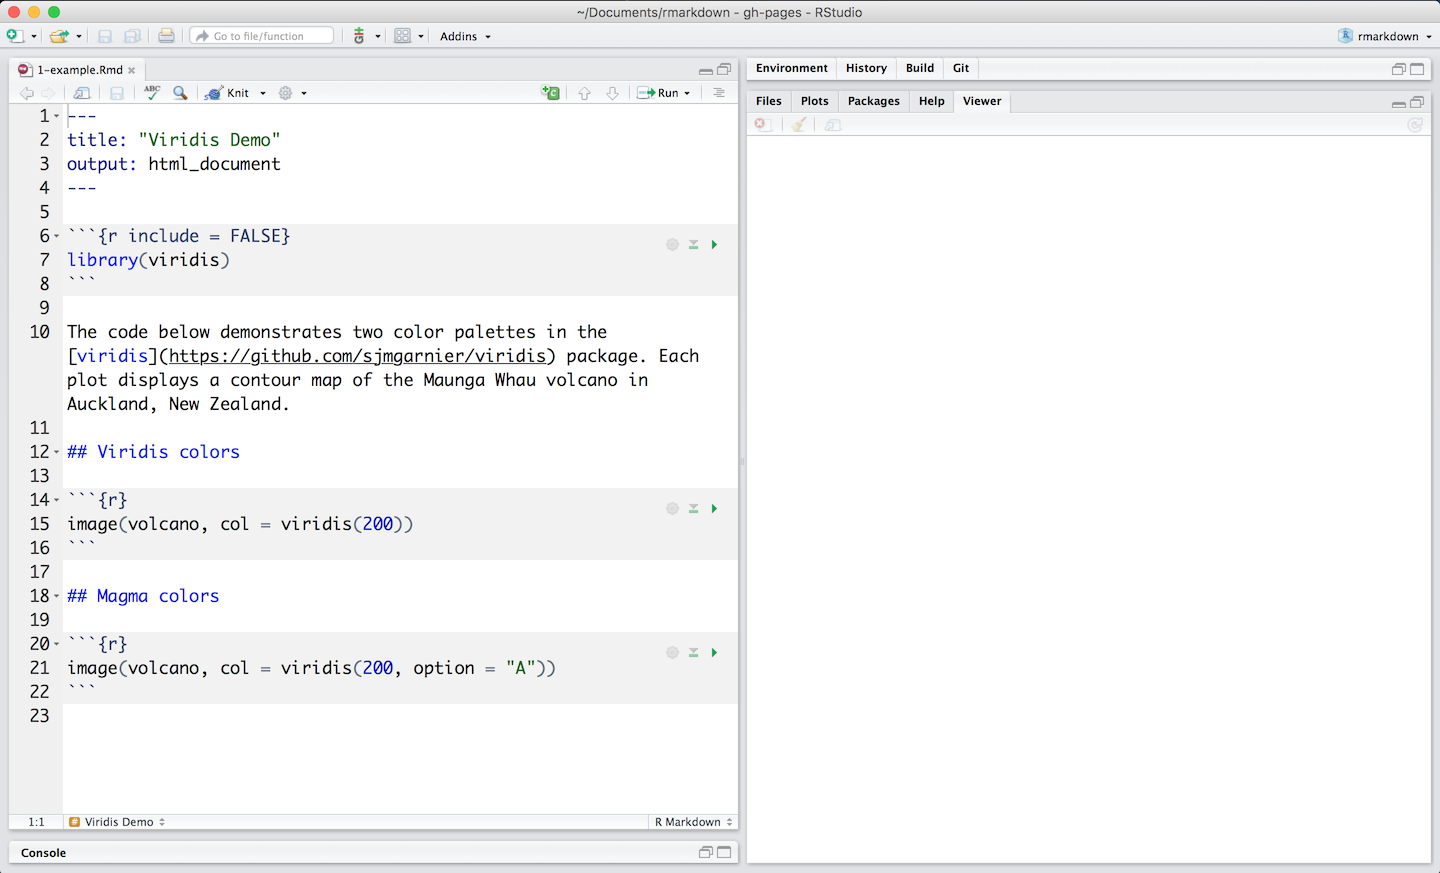
\includegraphics[width=5.20833in,height=\textheight]{images/rmarkdown/how-1-file.png}

Quarto 문서에는 주로 세 가지 유형의 컨텐츠가 포함됩니다. 첫째, YAML
헤더는 문서의 메타데이터를 정의하며, JSON처럼 데이터를 저장하는 데
사용됩니다. 둘째, 코드 청크는 백틱(```)으로 둘러싸여 있으며, R, Python
등의 다양한 언어 코드를 실행할 수 있습니다. 셋째, 일반 텍스트와 마크다운
문법으로 작성된 내용입니다.

\begin{verbatim}
---
title: "Lecture"
format: 
  html:
    toc: true
    toc-floating: true
    toc-depth: 2
    number-sections: true
---
\end{verbatim}

이러한 Quarto 파일은 \texttt{render}라는 명령어로 원하는 포맷의 문서로
변환할 수 있습니다. 아래 화면은 기본 Quarto 문서 생성시 보여지는
내용이며 html 형식으로 rendering 하기 위해서는 YAML에 html 임을 명시하고
아래와 같이 \texttt{render}함수를 사용하면 됩니다. 또는 Rstudio 코드
입력창 상단의 \texttt{Render} 버튼으로 pdf나 html 문서를 생성할 수
있습니다.

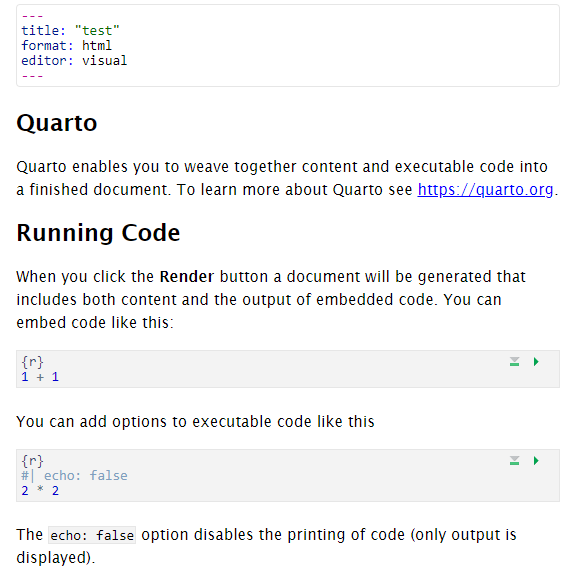
\includegraphics[width=4.20833in,height=\textheight]{images/image-1500245979.png}

Quarto는 내부적으로 \href{https://yihui.org/knitr/}{knitr} 패키지를
사용하여 R 및 기타 언어의 코드를 실행하여 .md 파일로 변환하고 .md 파일은
\href{https://pandoc.org/}{pandoc}을 통해 HTML, PDF, Word 등 다양한
형식의 문서로 최종 변환됩니다

\begin{Shaded}
\begin{Highlighting}[]
\InformationTok{\textasciigrave{}\textasciigrave{}\textasciigrave{}\{r\}}
\CommentTok{\#| eval=F}

\NormalTok{quarto}\SpecialCharTok{::}\FunctionTok{quarto\_render}\NormalTok{(}\StringTok{"test.qmd"}\NormalTok{, }\AttributeTok{output\_format =} \StringTok{"html"}\NormalTok{)}
\InformationTok{\textasciigrave{}\textasciigrave{}\textasciigrave{}}
\end{Highlighting}
\end{Shaded}

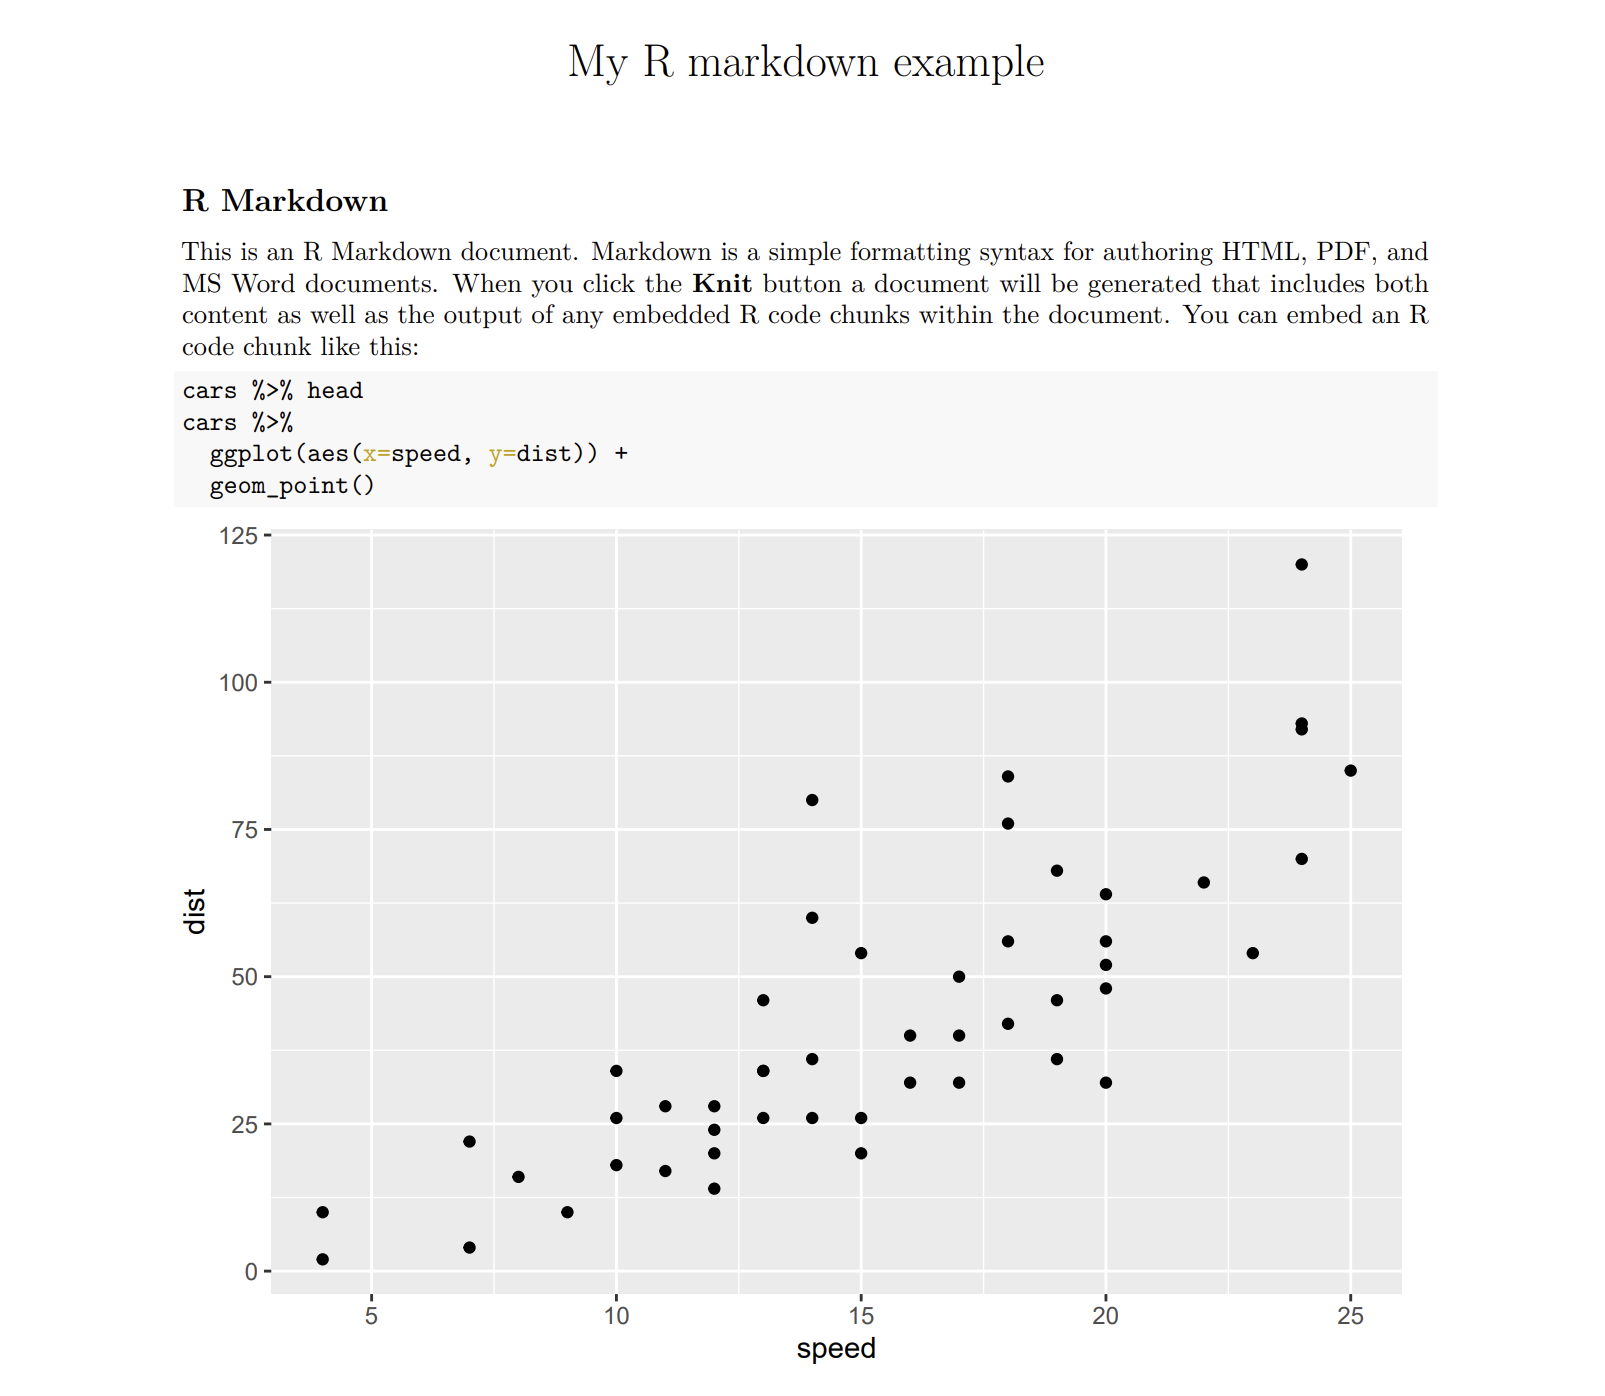
\includegraphics[width=3.59375in,height=\textheight]{images/rmarkdown/ex_pdf.PNG}

\hypertarget{uxcf54uxb4dc-uxc785uxb825}{%
\section{코드 입력}\label{uxcf54uxb4dc-uxc785uxb825}}

Quarto에서 코드 청크를 삽입하는 방법은 다음과 같습니다. 단축키
\texttt{Ctrl\ +\ Alt\ +\ I} (Windows) 또는 \texttt{Cmd\ +\ Option\ +\ I}
(macOS)를 사용할 수 있습니다. 코드 청크의 실행과 표시 여부를 결정하는
옵션을 다음과 같이 사용할 수 있습니다:

\begin{itemize}
\tightlist
\item
  \texttt{include:\ false} - 코드는 실행되지만 결과와 코드를 문서에
  표시하지 않습니다.
\item
  \texttt{echo:\ false} - 코드는 실행되고 결과가 포함되지만 코드는
  숨깁니다.
\item
  \texttt{eval:\ false} - 코드를 실행하지 않고 문서에만 표시합니다.
\item
  \texttt{message:\ false}, \texttt{warning:\ false},
  \texttt{error:\ false} - 코드 실행 중 발생하는 메시지, 경고, 에러를
  숨깁니다.
\item
  \texttt{fig.cap:\ "..."} - 코드로 생성된 그림에 캡션을 추가합니다.
\end{itemize}

R 코드 청크 예시:

코드는 실행되지만 결과와 코드를 표시하지 않습니다.

\begin{Shaded}
\begin{Highlighting}[]
\InformationTok{\textasciigrave{}\textasciigrave{}\textasciigrave{}\{r\}}
\CommentTok{\#| include=FALSE}

\FunctionTok{summary}\NormalTok{(cars)}
\InformationTok{\textasciigrave{}\textasciigrave{}\textasciigrave{}}
\end{Highlighting}
\end{Shaded}

코드는 실행되고 결과가 포함되지만 코드는 숨깁니다.

\begin{Shaded}
\begin{Highlighting}[]
\InformationTok{\textasciigrave{}\textasciigrave{}\textasciigrave{}\{r\}}
\CommentTok{\#| echo=FALSE}

\FunctionTok{summary}\NormalTok{(cars)}
\InformationTok{\textasciigrave{}\textasciigrave{}\textasciigrave{}}
\end{Highlighting}
\end{Shaded}

코드를 실행하지 않고 문서에만 표시합니다.

\begin{Shaded}
\begin{Highlighting}[]
\InformationTok{\textasciigrave{}\textasciigrave{}\textasciigrave{}\{r\}}
\CommentTok{\#| eval=FALSE}

\FunctionTok{summary}\NormalTok{(cars)}
\InformationTok{\textasciigrave{}\textasciigrave{}\textasciigrave{}}
\end{Highlighting}
\end{Shaded}

Python 코드 청크 예시:

\begin{Shaded}
\begin{Highlighting}[]
\InformationTok{\textasciigrave{}\textasciigrave{}\textasciigrave{}\{python\}}
\CommentTok{\#| eval: false}
\NormalTok{x }\OperatorTok{=} \StringTok{"hello, python in Quarto"}
\BuiltInTok{print}\NormalTok{(x.split(}\StringTok{\textquotesingle{} \textquotesingle{}}\NormalTok{))}
\InformationTok{\textasciigrave{}\textasciigrave{}\textasciigrave{}}
\end{Highlighting}
\end{Shaded}

Quarto 문서에서 코드 청크와 마크다운 문법을 사용하여 내용을 서식화하고
다양한 프로그래밍 언어의 코드를 실행할 수 있습니다. Quarto에 대한 자세한
정보와 사용법은 Quarto 공식 문서에서 확인할 수 있습니다.

Quarto에서는 `r~` 을 사용해서 코드청크가 아닌 곳에 R 코드를 넣을 수
있습니다
(\href{https://quarto.org/docs/get-started/computations/rstudio.html\#inline-code}{Inline
code}). 또한 R 언어 외에도 \texttt{Python}, \texttt{SQL}, \texttt{Bash},
\texttt{Rcpp}, \texttt{Stan}, \texttt{JavaScript}, \texttt{CSS} 등의
다양한 프로그래밍 언어에 대해서도 코드청크 기능을 사용할 수 있습니다.
그런데 이러한 언어들이 사용 가능해지기 위해서는 해당 언어들을 실행해주는
엔진이 (인터프리터) 있어야 하며 python의 경우 \texttt{reticulate} 라는
패키지가 이러한 기능을 담당합니다. 이 패키지를 설치할 경우
\texttt{miniconda}라는 가상환경 및 데이터 분석을 위한 오픈소스 패키지가
자동으로 설치됩니다.

\begin{Shaded}
\begin{Highlighting}[]
\InformationTok{\textasciigrave{}\textasciigrave{}\textasciigrave{}\{r\}}
\CommentTok{\#| eval: false}
\FunctionTok{library}\NormalTok{(reticulate)}
\InformationTok{\textasciigrave{}\textasciigrave{}\textasciigrave{}}
\end{Highlighting}
\end{Shaded}

위 \texttt{reticulate} 라이브러리를 로딩 후 아래 python 코드청크를
실행시킬 수 있습니다.

\begin{Shaded}
\begin{Highlighting}[]
\InformationTok{\textasciigrave{}\textasciigrave{}\textasciigrave{}\{python\}}
\CommentTok{\#| eval: false}
\NormalTok{x }\OperatorTok{=} \StringTok{"hello, python in R"}
\BuiltInTok{print}\NormalTok{(x.split(}\StringTok{\textquotesingle{} \textquotesingle{}}\NormalTok{))}
\InformationTok{\textasciigrave{}\textasciigrave{}\textasciigrave{}}
\end{Highlighting}
\end{Shaded}

\hypertarget{markdown-uxbb38uxbc95}{%
\section{Markdown 문법}\label{markdown-uxbb38uxbc95}}

마크다운은 plain text 기반의 마크업 언어로서 마크업 언어는 태그 등을
이용해서 문서의 데이터 구조를 명시하는데 이러한 태그를 사용하는 방법
체계를 마크업 언어라고 합니다. 가장 대표적으로 html 이 있습니다.

\begin{verbatim}
    <html>
      <head>
        <title> Hello HTML </title>
      </head>
      <body>
      Hello markup world!
      </body>
    </html>
\end{verbatim}

마크다운도 몇 가지 태그를 이용해서 문서의 구조를 정의하고 있으며 상세한
내용은
\href{https://rmarkdown.rstudio.com/authoring_pandoc_markdown.html}{Pandoc
마크다운 문서}를 참고하시기 바랍니다. 마크다운언어의 철학은 쉽게 읽고 쓸
수 있는 문서입니다. plain text 기반으로 작성되어 쓰기 쉬우며 (아직도
사람들이 메모장 많이 사용하는 이유와 같습니다) 태그가 포함되어 있어도
읽는데 어려움이 없습니다. 위 html 언어와 아래 markdown 파일의 예들을
보시면 그 차이를 어렵지 않게 이해할 수 있습니다.

마크다운에서는 Enter를 한 번 입력해서 줄바꿈이 되지 않습니다.
\texttt{\textless{}br\textgreater{}} 또는 문장 마지막에 공백을 두 개
입력하면 되겠습니다.

\begin{verbatim}
    이 분장은 줄바꿈이<br>
    됩니다
\end{verbatim}

마크다운 테그를 몇 가지 살펴보면 먼저 \# 을 붙여서 만드는 header 가
있습니다.

\begin{verbatim}
    # A level-one header
    ## A level-two header
    ### A level-three header

    # A level-one header {#l1-1}
    ## A level-two header {#l2-1}
    ### A level-three header {#l3-1}

    # A level-one header {#l1-2}
    ## A level-two header {#l2-2}
    ### A level-three header {#l3-2}
\end{verbatim}

인용문구를 나타내는 Block quotations이 있습니다.

\begin{quote}
This is block quote. This paragraph has two lines
\end{quote}

\begin{verbatim}
    > This is block quote. This paragraph has two lines
\end{verbatim}

\begin{quote}
This is a block quote.

\begin{quote}
A block quote within a block quote.
\end{quote}
\end{quote}

\begin{verbatim}
    > This is a block quote.
    >
    > > A block quote within a block quote.
\end{verbatim}

\emph{Italic}

\begin{verbatim}
    *Italic*
\end{verbatim}

\textbf{Bold}

\begin{verbatim}
    **Bold**
\end{verbatim}

\href{https://www.naver.com/}{Naver link}

\begin{verbatim}
    [Naver link](https://www.naver.com/)
\end{verbatim}

이미지를 직접 삽입하고 가운데 정렬합니다.

\begin{figure}

{\centering 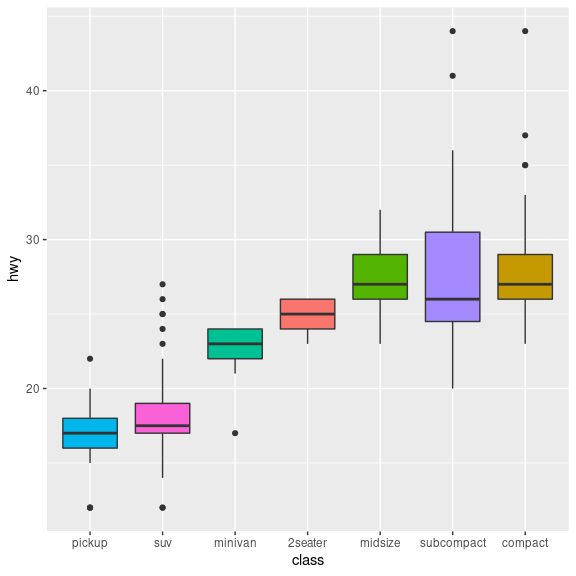
\includegraphics[width=2.08333in,height=\textheight]{images/rmarkdown/000002.png}

}

\caption{자동차 모델에 따른 고속도로 연비 분포}

\end{figure}

\begin{verbatim}
    <center>
    ![자동차 모델에 따른 고속도로 연비 분포](images/rmarkdown/000002.png){width="200"}
    </center>
\end{verbatim}

\textbf{Lists:}

순서형 리스트는 숫자 해더를 사용하고 비순서형 리스트는 dash나 다른
bullet 포인트를 사용합니다.

\begin{enumerate}
\def\labelenumi{\arabic{enumi}.}
\tightlist
\item
  첫 번째
\item
  두 번째
\item
  세 번째
\end{enumerate}

\begin{itemize}
\tightlist
\item
  아이템 1
\item
  아이템 2
\item
  아이템 3

  \begin{itemize}
  \tightlist
  \item
    아이템 3-1
  \item
    아이템 3-2
  \end{itemize}
\end{itemize}

\begin{verbatim}

    1.  첫 번째
    2.  두 번째
    3.  세 번째
    
    -   아이템 1
    -   아이템 2
    -   아이템 3
        -   아이템 3-1
        -   아이템 3-2
\end{verbatim}

참고로 소스코드 그대로 표현하기 위해서는
\texttt{\#\textbar{}\ echo:\ fanced} 를 사용하거나 두 개의 중괄호 (curly
braces)를
(\href{https://quarto.org/docs/computations/execution-options.html\#fenced-echo}{fanced
echo 도움말}) 사용하며 일반 택스트의 경우는 백틱 세 개나 (```)
들여쓰기를 사용합니다.

\hypertarget{uxc2a4uxd0c0uxc77c}{%
\section{스타일}\label{uxc2a4uxd0c0uxc77c}}

아래와 같이 YAML 해더에 css파일을 삽입하고 해당되는 class 또는 id에
해당하는 내용에 스타일을 적용할 수 있습니다.

\textbf{style.css}

\begin{verbatim}
    .header1 {
    color: red;
    }
\end{verbatim}

위와 같이 style.css 파일 작성 후 quarto파일에서 다음과 같이 사용

\begin{Shaded}
\begin{Highlighting}[]
\InformationTok{    {-}{-}{-}}
\InformationTok{    title: "test"}
\InformationTok{    format:}
\InformationTok{      html:}
\InformationTok{        css: styles.css}
\InformationTok{    {-}{-}{-}}
\InformationTok{    }
\InformationTok{    \textasciigrave{}\textasciigrave{}\textasciigrave{}\{r\}}
\InformationTok{    \#| classes: header}
\InformationTok{    }
\InformationTok{    2 + 2}
\InformationTok{    \textasciigrave{}\textasciigrave{}\textasciigrave{}}
\end{Highlighting}
\end{Shaded}

\hypertarget{uxd14cuxc774uxbe14}{%
\section{테이블}\label{uxd14cuxc774uxbe14}}

\texttt{kable} 함수를 이용하여 Quarto 문서에 포함되는 표를 원하는
방향으로 작성할 수 있습니다. \texttt{mtcars}는 데이터프레임 형식의
데이터입니다.

\begin{Shaded}
\begin{Highlighting}[]
\NormalTok{knitr}\SpecialCharTok{::}\FunctionTok{kable}\NormalTok{(}
\NormalTok{  mtcars[}\DecValTok{1}\SpecialCharTok{:}\DecValTok{5}\NormalTok{, ], }
  \AttributeTok{caption =} \StringTok{"A knitr kable."}
\NormalTok{)}
\end{Highlighting}
\end{Shaded}

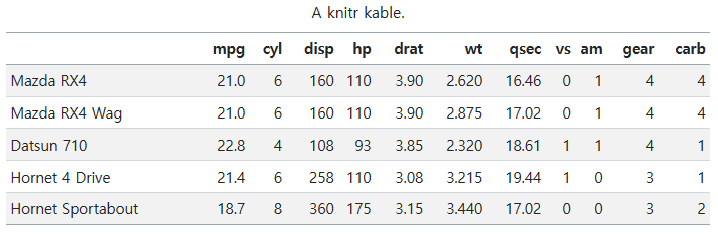
\includegraphics{images/image-597049431.png}

\hypertarget{yaml-uxd5e4uxb354}{%
\section{YAML 헤더}\label{yaml-uxd5e4uxb354}}

Quarto 파일에서 YAML의 가장 중요한 기능은 output 포멧을 지정하는 것이며
title, author, date, 등을 설정할수도 있습니다.

\begin{verbatim}
    ---
    title: "R Programming"
    subtitle: "Using Quarto"
    format:
      html:
        css: style.css
        includes:
          in_header: header.html
          after_body: footer.html
        toc: true
        toc_float: true
        number_sections: true
    mainfont: NanumGothic
    ---
\end{verbatim}

\hypertarget{output-format}{%
\section{Output format}\label{output-format}}

Quarto의 output format 설정은 사용자가 만드는 문서의 종류와 필요에 맞게
유연하게 조정할 수 있으며, 이를 통해 다양한 형식의 고품질 문서를 생성할
수 있습니다. Quarto 문서에 대한 보다 자세한 정보는
\href{https://quarto.org/docs/guide/}{Quarto 공식 문서}에서 확인할 수
있습니다.

\hypertarget{uxc5f0uxc2b5uxbb38uxc81c}{%
\section{연습문제}\label{uxc5f0uxc2b5uxbb38uxc81c}}

\hypertarget{uxc5f0uxc2b5uxbb38uxc81c-1-uxae30uxbcf8-html-uxbb38uxc11c-uxc0dduxc131}{%
\subsection{연습문제 1: 기본 HTML 문서
생성}\label{uxc5f0uxc2b5uxbb38uxc81c-1-uxae30uxbcf8-html-uxbb38uxc11c-uxc0dduxc131}}

Quarto를 사용하여 간단한 HTML 문서를 생성합니다. 이 문서에는 자기 소개,
몇 개의 섹션, 그리고 R 코드 청크가 포함되어야 합니다.

\begin{itemize}
\item
  새 Quarto 문서 생성
\item
  문서의 제목을 ``My Quarto''로 설정
\item
  YAML 헤더에 \textbf{\texttt{format:\ html}} 추가
\item
  마크다운 언어로 자기소개 섹션과 데이터 분석 섹션 추가
\item
  ``데이터 분석'' 섹션에 \textbf{\texttt{mtcars}} 데이터셋의 요약 통계를
  보여주는 코드 청크를 포함

\begin{verbatim}
summary(mtcars)
\end{verbatim}
\end{itemize}

\hypertarget{uxc5f0uxc2b5uxbb38uxc81c-2-uxc2acuxb77cuxc774uxb4dc-uxc1fc-uxc0dduxc131}{%
\subsection{연습문제 2: 슬라이드 쇼
생성}\label{uxc5f0uxc2b5uxbb38uxc81c-2-uxc2acuxb77cuxc774uxb4dc-uxc1fc-uxc0dduxc131}}

Quarto를 사용하여 간단한 슬라이드 쇼를 생성합니다. 이 슬라이드 쇼에는
여러 개의 슬라이드와 최소 하나의 인터랙티브한 R 코드 청크가 포함되어야
합니다.

\begin{itemize}
\item
  새 Quarto 문서를 생성하고 파일 이름을 ``슬라이드 쇼 연습''으로 설정
\item
  YAML 헤더에 \textbf{\texttt{format:\ revealjs}} 추가
\item
  첫 번째 슬라이드에는 간단한 소개 및 슬라이드 쇼의 주제 작성
\item
  두 번째 슬라이드에는 \textbf{\texttt{ggplot2}} 사용한
  \textbf{\texttt{mtcars}} 데이터셋의 \textbf{\texttt{mpg}}
  vs.~\textbf{\texttt{cyl}} 그래프 표시

\begin{verbatim}
library(ggplot2)
ggplot(mtcars, aes(x=cyl, y=mpg)) + geom_point()
\end{verbatim}
\item
  세 번째 슬라이드에는 결론 및 요약 포함
\end{itemize}

\begin{center}\rule{0.5\linewidth}{0.5pt}\end{center}

이 저작물은 크리에이티브 커먼즈 저작자표시-비영리-변경금지 4.0 국제
라이선스에 따라 이용할 수 있습니다.

\bookmarksetup{startatroot}

\hypertarget{data-transformation-classic}{%
\chapter{Data transformation
classic}\label{data-transformation-classic}}

\hypertarget{introduction-2}{%
\section{Introduction}\label{introduction-2}}

Quarto는 데이터 과학에서 사용되는 코드와 리포트를 결합할 수 있는 통합
문서 시스템입니다. 마이크로소프트 워드나 한글과 같은 워드 프로세서에서
프로그래밍 코드와 데이터 분석을 수행할 수 있는 것처럼, Quarto를 사용하면
텍스트 기반의 마크다운 문법으로 문서를 작성하고 다양한 형식의 출력물로
변환할 수 있습니다. 이러한 출력물에는 HTML, PDF, Word 문서, 슬라이드 쇼,
책, 웹사이트 등이 포함됩니다.

Quarto에 대한 더 자세한 정보는 Quarto 공식 웹사이트에서 확인할 수
있습니다. 해당 웹사이트에는 Quarto 소개 동영상과
\href{https://quarto.org/docs/}{Quarto 공식 사이트 메뉴얼}이 있으며,
Quarto를 사용할 때 참고할 수 있는
\href{https://quarto.org/docs/cheatsheets/quarto}{cheatsheet}도
제공됩니다.

\hypertarget{quartouxc758-uxae30uxbcf8-uxc791uxb3d9-uxc6d0uxb9ac-1}{%
\section{Quarto의 기본 작동
원리}\label{quartouxc758-uxae30uxbcf8-uxc791uxb3d9-uxc6d0uxb9ac-1}}

Quarto는 plain text 기반으로 작성되며 \texttt{.qmd} 라는 확장자를 갖는
파일로 저장됩니다. 다음과 같은 텍스트 파일이 Quarto 파일의 전형적인
예입니다.

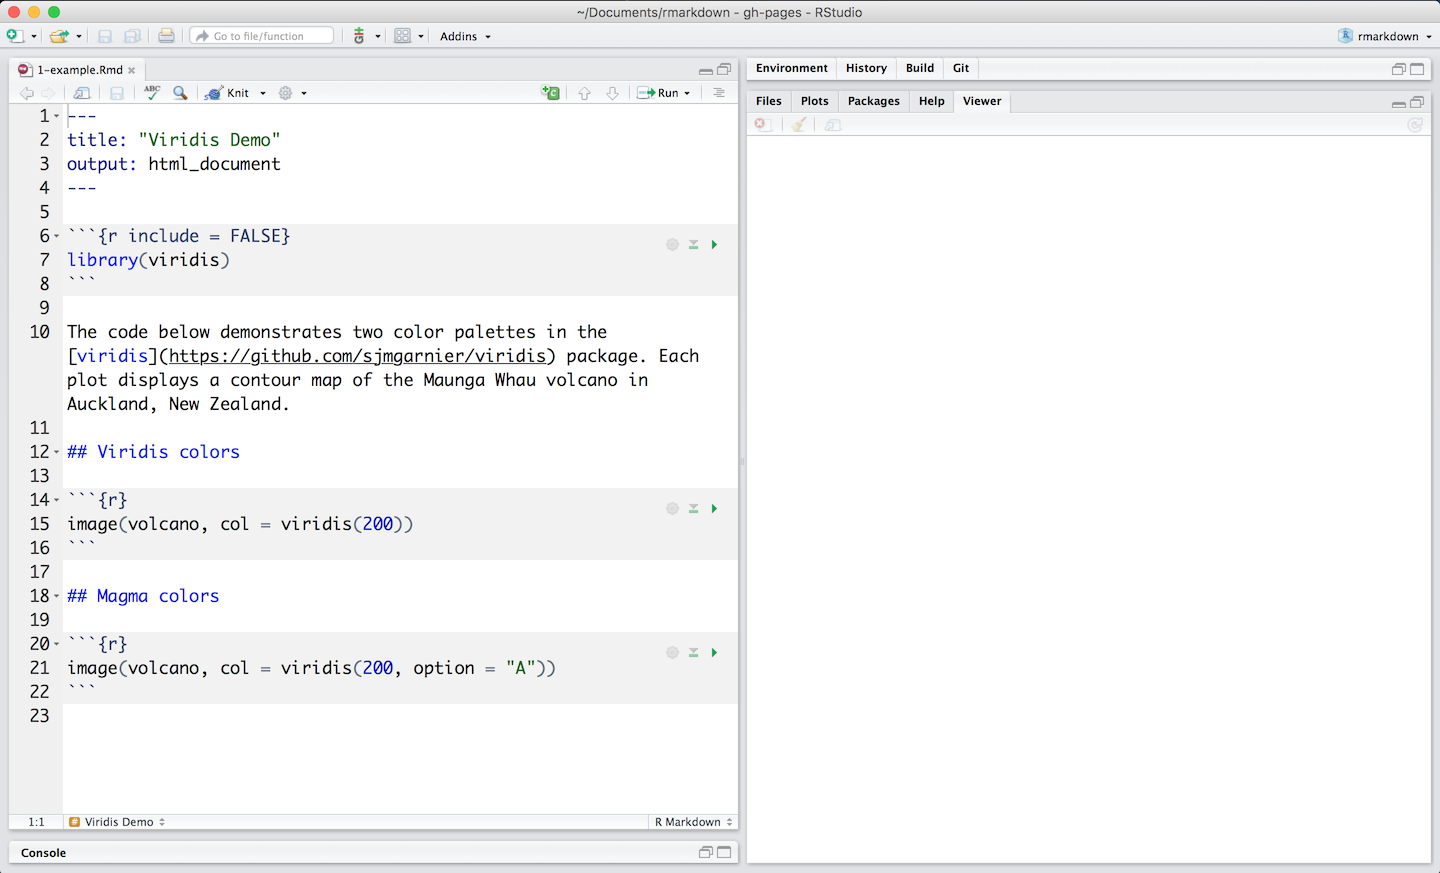
\includegraphics[width=5.20833in,height=\textheight]{images/rmarkdown/how-1-file.png}

Quarto 문서에는 주로 세 가지 유형의 컨텐츠가 포함됩니다. 첫째, YAML
헤더는 문서의 메타데이터를 정의하며, JSON처럼 데이터를 저장하는 데
사용됩니다. 둘째, 코드 청크는 백틱(```)으로 둘러싸여 있으며, R, Python
등의 다양한 언어 코드를 실행할 수 있습니다. 셋째, 일반 텍스트와 마크다운
문법으로 작성된 내용입니다.

\begin{verbatim}
---
title: "Lecture"
format: 
  html:
    toc: true
    toc-floating: true
    toc-depth: 2
    number-sections: true
---
\end{verbatim}

이러한 Quarto 파일은 \texttt{render}라는 명령어로 원하는 포맷의 문서로
변환할 수 있습니다. 다음 예의 파일을 html 형식으로 rendering 하기
위해서는 YAML에 html 임을 명시하고 아래와 같이 \texttt{render}함수를
사용하면 됩니다. 또는 Rstudio 코드 입력창 상단의 Knit 버튼으로 pdf나
html 문서를 생성할 수 있습니다.

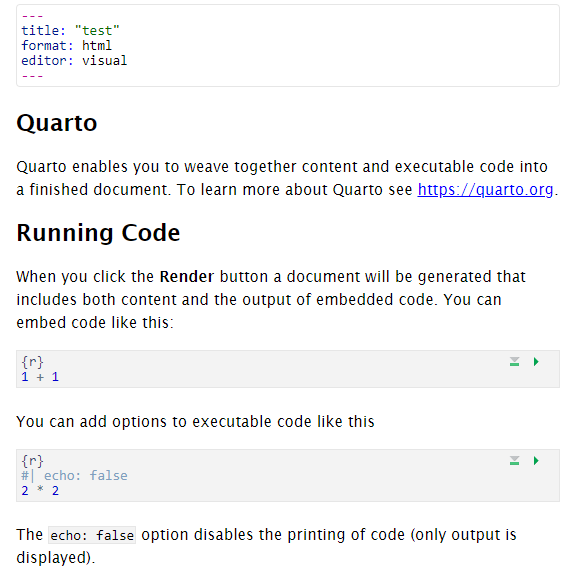
\includegraphics[width=4.20833in,height=\textheight]{images/image-1500245979.png}

Quarto는 내부적으로 \href{https://yihui.org/knitr/}{knitr} 패키지를
사용하여 R 및 기타 언어의 코드를 실행하여 .md 파일로 변환하고 .md 파일은
\href{https://pandoc.org/}{pandoc}을 통해 HTML, PDF, Word 등 다양한
형식의 문서로 최종 변환됩니다

\begin{Shaded}
\begin{Highlighting}[]
\NormalTok{quarto}\SpecialCharTok{::}\FunctionTok{quarto\_render}\NormalTok{(}\StringTok{"test.qmd"}\NormalTok{, }\AttributeTok{output\_format =} \StringTok{"html"}\NormalTok{)}
\end{Highlighting}
\end{Shaded}

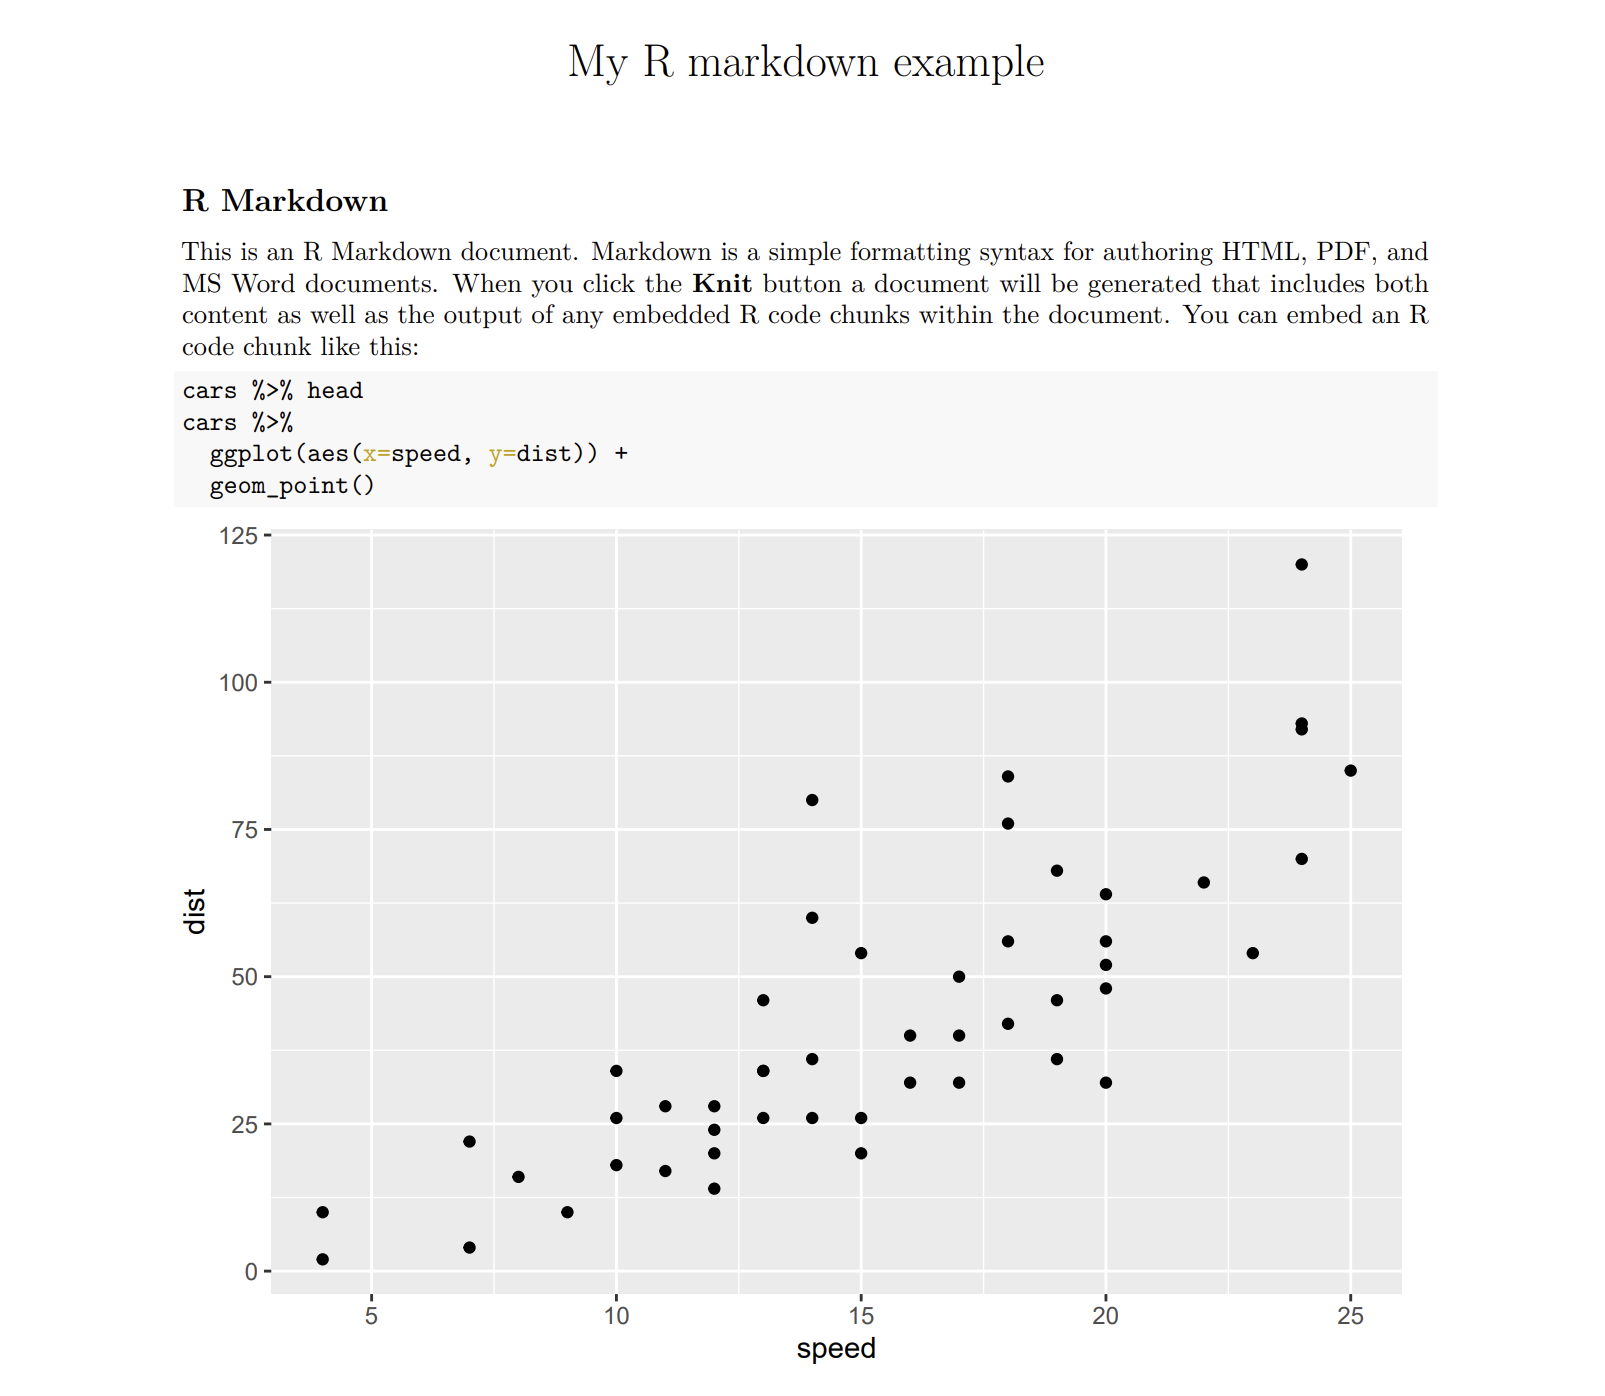
\includegraphics[width=3.59375in,height=\textheight]{images/rmarkdown/ex_pdf.PNG}

\hypertarget{uxcf54uxb4dc-uxc785uxb825-1}{%
\section{코드 입력}\label{uxcf54uxb4dc-uxc785uxb825-1}}

Quarto에서 코드 청크를 삽입하는 방법은 다음과 같습니다. 단축키
\texttt{Ctrl\ +\ Alt\ +\ I} (Windows) 또는 \texttt{Cmd\ +\ Option\ +\ I}
(macOS)를 사용할 수 있습니다. 코드 청크의 실행과 표시 여부를 결정하는
옵션을 다음과 같이 사용할 수 있습니다:

\begin{itemize}
\tightlist
\item
  \texttt{include:\ false} - 코드는 실행되지만 결과와 코드를 문서에
  표시하지 않습니다.
\item
  \texttt{echo:\ false} - 코드는 실행되고 결과가 포함되지만 코드는
  숨깁니다.
\item
  \texttt{eval:\ false} - 코드를 실행하지 않고 문서에만 표시합니다.
\item
  \texttt{message:\ false}, \texttt{warning:\ false},
  \texttt{error:\ false} - 코드 실행 중 발생하는 메시지, 경고, 에러를
  숨깁니다.
\item
  \texttt{fig.cap:\ "..."} - 코드로 생성된 그림에 캡션을 추가합니다.
\end{itemize}

R 코드 청크 예시:

코드는 실행되지만 결과와 코드를 표시하지 않습니다.

코드는 실행되고 결과가 포함되지만 코드는 숨깁니다.

\begin{verbatim}
::: {.cell}
::: {.cell-output .cell-output-stdout}
```
     speed           dist       
 Min.   : 4.0   Min.   :  2.00  
 1st Qu.:12.0   1st Qu.: 26.00  
 Median :15.0   Median : 36.00  
 Mean   :15.4   Mean   : 42.98  
 3rd Qu.:19.0   3rd Qu.: 56.00  
 Max.   :25.0   Max.   :120.00  
```
:::
:::
\end{verbatim}

코드를 실행하지 않고 문서에만 표시합니다.

\begin{verbatim}
::: {.cell}

```{.r .cell-code}
summary(cars)
```
:::
\end{verbatim}

Python 코드 청크 예시:

\begin{Shaded}
\begin{Highlighting}[]
\NormalTok{x }\OperatorTok{=} \StringTok{"hello, python in Quarto"}
\BuiltInTok{print}\NormalTok{(x.split(}\StringTok{\textquotesingle{} \textquotesingle{}}\NormalTok{))}
\end{Highlighting}
\end{Shaded}

Quarto 문서에서 코드 청크와 마크다운 문법을 사용하여 내용을 서식화하고
다양한 프로그래밍 언어의 코드를 실행할 수 있습니다. Quarto에 대한 자세한
정보와 사용법은 Quarto 공식 문서에서 확인할 수 있습니다.

Quarto에서는 ` r`을 사용해서 코드청크가 아닌 곳에 R 코드를 넣을 수
있습니다. 또한 R 언어 외에도 \texttt{Python}, \texttt{SQL},
\texttt{Bash}, \texttt{Rcpp}, \texttt{Stan}, \texttt{JavaScript},
\texttt{CSS} 등의 다양한 프로그래밍 언어에 대해서도 코드청크 기능을
사용할 수 있습니다. 그런데 이러한 언어들이 사용 가능해지기 위해서는 해당
언어들을 실행해주는 엔진이 (인터프리터) 있어야 하며 python의 경우
\texttt{reticulate} 라는 패키지가 이러한 기능을 담당합니다. 이 패키지를
설치할 경우 \texttt{miniconda}라는 가상환경 및 데이터 분석을 위한
오픈소스 패키지가 자동으로 설치됩니다.

\begin{Shaded}
\begin{Highlighting}[]
\FunctionTok{library}\NormalTok{(reticulate)}
\end{Highlighting}
\end{Shaded}

\begin{Shaded}
\begin{Highlighting}[]
\NormalTok{x }\OperatorTok{=} \StringTok{"hello, python in R"}
\BuiltInTok{print}\NormalTok{(x.split(}\StringTok{\textquotesingle{} \textquotesingle{}}\NormalTok{))}
\end{Highlighting}
\end{Shaded}

\hypertarget{markdown-uxbb38uxbc95-1}{%
\section{Markdown 문법}\label{markdown-uxbb38uxbc95-1}}

마크다운은 plain text 기반의 마크업 언어로서 마크업 언어는 태그 등을
이용해서 문서의 데이터 구조를 명시하는데 이러한 태그를 사용하는 방법
체계를 마크업 언어라고 합니다. 가장 대표적으로 html 이 있습니다.

\begin{verbatim}
    <html>
      <head>
        <title> Hello HTML </title>
      </head>
      <body>
      Hello markup world!
      </body>
    </html>
\end{verbatim}

마크다운도 몇 가지 태그를 이용해서 문서의 구조를 정의하고 있으며 상세한
내용은
\href{https://rmarkdown.rstudio.com/authoring_pandoc_markdown.html}{Pandoc
마크다운 문서}를 참고하시기 바랍니다. 마크다운언어의 철학은 쉽게 읽고 쓸
수 있는 문서입니다. plain text 기반으로 작성되어 쓰기 쉬우며 (아직도
사람들이 메모장 많이 사용하는 이유와 같습니다) 태그가 포함되어 있어도
읽는데 어려움이 없습니다. 위 html 언어와 아래 markdown 파일의 예들을
보시면 그 차이를 어렵지 않게 이해할 수 있습니다.

마크다운에서는 Enter를 한 번 입력해서 줄바꿈이 되지 않습니다.
\texttt{\textless{}br\textgreater{}} 또는 문장 마지막에 공백을 두 개
입력하면 되겠습니다.

\begin{verbatim}
이 문장은 줄바꿈이 
되지 않습니다
\end{verbatim}

이 문장은 줄바꿈이 되지 않습니다

\begin{verbatim}
이 분장은 줄바꿈이<br>
됩니다
\end{verbatim}

이 분장은 줄바꿈이 됩니다

마크다운 테그를 몇 가지 살펴보면 먼저 \# 을 붙여서 만드는 header 가
있습니다.

\begin{verbatim}
# A level-one header
## A level-two header
### A level-three header

# A level-one header {#l1-1}
## A level-two header {#l2-1}
### A level-three header {#l3-1}

# A level-one header {#l1-2}
## A level-two header {#l2-2}
### A level-three header {#l3-2}
\end{verbatim}

Block quotations

\begin{quote}
This is block quote. This paragraph has two lines
\end{quote}

\begin{verbatim}
> This is block quote. This paragraph has two lines
\end{verbatim}

\begin{quote}
This is a block quote.

\begin{quote}
A block quote within a block quote.
\end{quote}
\end{quote}

\begin{verbatim}
> This is a block quote.
>
> > A block quote within a block quote.
\end{verbatim}

\emph{Italic}

\begin{verbatim}
*Italic*
\end{verbatim}

\textbf{Bold}

\begin{verbatim}
**Bold**
\end{verbatim}

\href{https://www.naver.com/}{Naver link}

\begin{verbatim}
[Naver link](https://www.naver.com/)
\end{verbatim}

이미지를 직접 삽입하고 가운데 정렬합니다.

\begin{figure}

{\centering 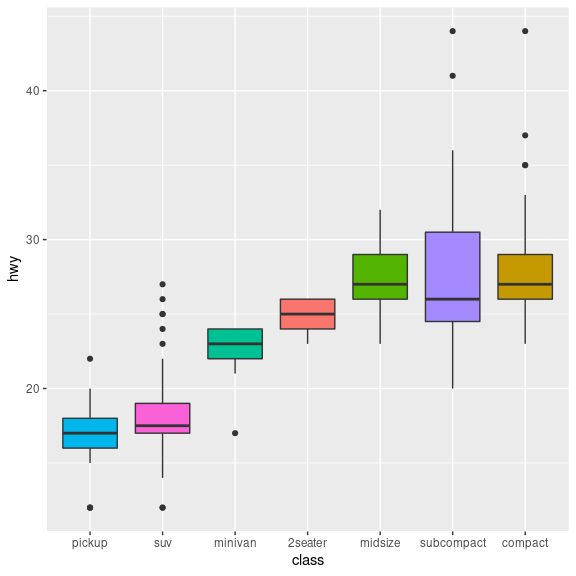
\includegraphics[width=2.08333in,height=\textheight]{images/rmarkdown/000002.png}

}

\caption{자동차 모델에 따른 고속도로 연비 분포}

\end{figure}

\begin{verbatim}
<center>
![자동차 모델에 따른 고속도로 연비 분포](images/rmarkdown/000002.png){width="200"}
</center>
\end{verbatim}

\textbf{Lists:}

순서형 리스트는 숫자 해더를 사용하고 비순서형 리스트는 dash나 다른
bullet 포인트를 사용합니다.

\begin{verbatim}
    1.  첫 번째
    2.  두 번째
    3.  세 번째

    -   아이템 1
    -   아이템 2
    -   아이템 3
        -   아이템 3-1
        -   아이템 3-2
\end{verbatim}

참고로 소스코드 그대로 표현하기 위해서는 백틱 세 개나 (```) 들여쓰기 두
칸을 사용합니다.

\hypertarget{uxc2a4uxd0c0uxc77c-1}{%
\section{스타일}\label{uxc2a4uxd0c0uxc77c-1}}

아래와 같이 YAML 해더에 css파일을 삽입하고 해당되는 class 또는 id에
해당하는 내용에 스타일을 적용할 수 있습니다.

\textbf{style.css}

\begin{verbatim}
.header1 {
color: red;
}
\end{verbatim}

quarto파일에서 다음과 같이 사용

\begin{verbatim}
---
title: "test"
format:
  html:
    css: styles.css
---


::: {.cell .header}

```{.r .cell-code}
2 + 2
```

::: {.cell-output .cell-output-stdout}
```
[1] 4
```
:::
:::
\end{verbatim}

\hypertarget{uxd14cuxc774uxbe14-1}{%
\section{테이블}\label{uxd14cuxc774uxbe14-1}}

\texttt{kable} 함수를 이용하여 Quarto 문서에 포함되는 표를 원하는
방향으로 작성할 수 있습니다. \texttt{mtcars}는 데이터프레임 형식의
데이터입니다.

\begin{Shaded}
\begin{Highlighting}[]
\NormalTok{knitr}\SpecialCharTok{::}\FunctionTok{kable}\NormalTok{(}
\NormalTok{  mtcars[}\DecValTok{1}\SpecialCharTok{:}\DecValTok{5}\NormalTok{, ], }
  \AttributeTok{caption =} \StringTok{"A knitr kable."}
\NormalTok{)}
\end{Highlighting}
\end{Shaded}

\begin{longtable}[]{@{}
  >{\raggedright\arraybackslash}p{(\columnwidth - 22\tabcolsep) * \real{0.2609}}
  >{\raggedleft\arraybackslash}p{(\columnwidth - 22\tabcolsep) * \real{0.0725}}
  >{\raggedleft\arraybackslash}p{(\columnwidth - 22\tabcolsep) * \real{0.0580}}
  >{\raggedleft\arraybackslash}p{(\columnwidth - 22\tabcolsep) * \real{0.0725}}
  >{\raggedleft\arraybackslash}p{(\columnwidth - 22\tabcolsep) * \real{0.0580}}
  >{\raggedleft\arraybackslash}p{(\columnwidth - 22\tabcolsep) * \real{0.0725}}
  >{\raggedleft\arraybackslash}p{(\columnwidth - 22\tabcolsep) * \real{0.0870}}
  >{\raggedleft\arraybackslash}p{(\columnwidth - 22\tabcolsep) * \real{0.0870}}
  >{\raggedleft\arraybackslash}p{(\columnwidth - 22\tabcolsep) * \real{0.0435}}
  >{\raggedleft\arraybackslash}p{(\columnwidth - 22\tabcolsep) * \real{0.0435}}
  >{\raggedleft\arraybackslash}p{(\columnwidth - 22\tabcolsep) * \real{0.0725}}
  >{\raggedleft\arraybackslash}p{(\columnwidth - 22\tabcolsep) * \real{0.0725}}@{}}
\caption{A knitr kable.}\tabularnewline
\toprule\noalign{}
\begin{minipage}[b]{\linewidth}\raggedright
\end{minipage} & \begin{minipage}[b]{\linewidth}\raggedleft
mpg
\end{minipage} & \begin{minipage}[b]{\linewidth}\raggedleft
cyl
\end{minipage} & \begin{minipage}[b]{\linewidth}\raggedleft
disp
\end{minipage} & \begin{minipage}[b]{\linewidth}\raggedleft
hp
\end{minipage} & \begin{minipage}[b]{\linewidth}\raggedleft
drat
\end{minipage} & \begin{minipage}[b]{\linewidth}\raggedleft
wt
\end{minipage} & \begin{minipage}[b]{\linewidth}\raggedleft
qsec
\end{minipage} & \begin{minipage}[b]{\linewidth}\raggedleft
vs
\end{minipage} & \begin{minipage}[b]{\linewidth}\raggedleft
am
\end{minipage} & \begin{minipage}[b]{\linewidth}\raggedleft
gear
\end{minipage} & \begin{minipage}[b]{\linewidth}\raggedleft
carb
\end{minipage} \\
\midrule\noalign{}
\endfirsthead
\toprule\noalign{}
\begin{minipage}[b]{\linewidth}\raggedright
\end{minipage} & \begin{minipage}[b]{\linewidth}\raggedleft
mpg
\end{minipage} & \begin{minipage}[b]{\linewidth}\raggedleft
cyl
\end{minipage} & \begin{minipage}[b]{\linewidth}\raggedleft
disp
\end{minipage} & \begin{minipage}[b]{\linewidth}\raggedleft
hp
\end{minipage} & \begin{minipage}[b]{\linewidth}\raggedleft
drat
\end{minipage} & \begin{minipage}[b]{\linewidth}\raggedleft
wt
\end{minipage} & \begin{minipage}[b]{\linewidth}\raggedleft
qsec
\end{minipage} & \begin{minipage}[b]{\linewidth}\raggedleft
vs
\end{minipage} & \begin{minipage}[b]{\linewidth}\raggedleft
am
\end{minipage} & \begin{minipage}[b]{\linewidth}\raggedleft
gear
\end{minipage} & \begin{minipage}[b]{\linewidth}\raggedleft
carb
\end{minipage} \\
\midrule\noalign{}
\endhead
\bottomrule\noalign{}
\endlastfoot
Mazda RX4 & 21.0 & 6 & 160 & 110 & 3.90 & 2.620 & 16.46 & 0 & 1 & 4 &
4 \\
Mazda RX4 Wag & 21.0 & 6 & 160 & 110 & 3.90 & 2.875 & 17.02 & 0 & 1 & 4
& 4 \\
Datsun 710 & 22.8 & 4 & 108 & 93 & 3.85 & 2.320 & 18.61 & 1 & 1 & 4 &
1 \\
Hornet 4 Drive & 21.4 & 6 & 258 & 110 & 3.08 & 3.215 & 19.44 & 1 & 0 & 3
& 1 \\
Hornet Sportabout & 18.7 & 8 & 360 & 175 & 3.15 & 3.440 & 17.02 & 0 & 0
& 3 & 2 \\
\end{longtable}

\hypertarget{yaml-uxd5e4uxb354-1}{%
\section{YAML 헤더}\label{yaml-uxd5e4uxb354-1}}

Quarto 파일에서 YAML의 가장 중요한 기능은 output 포멧을 지정하는 것이며
title, author, date, 등을 설정할수도 있습니다.

\begin{verbatim}
    ---
    title: "R Programming"
    subtitle: "Using Quarto"
    format:
      html:
        css: style.css
        includes:
          in_header: header.html
          after_body: footer.html
        toc: true
        toc_float: true
        number_sections: true
    mainfont: NanumGothic
    ---
\end{verbatim}

\hypertarget{output-format-1}{%
\section{Output format}\label{output-format-1}}

Quarto의 output format 설정은 사용자가 만드는 문서의 종류와 필요에 맞게
유연하게 조정할 수 있으며, 이를 통해 다양한 형식의 고품질 문서를 생성할
수 있습니다. Quarto 문서에 대한 보다 자세한 정보는
\href{https://quarto.org/docs/guide/}{Quarto 공식 문서}에서 확인할 수
있습니다.

\hypertarget{uxc5f0uxc2b5uxbb38uxc81c-1}{%
\section{연습문제}\label{uxc5f0uxc2b5uxbb38uxc81c-1}}

\hypertarget{uxc5f0uxc2b5uxbb38uxc81c-1-uxae30uxbcf8-html-uxbb38uxc11c-uxc0dduxc131-1}{%
\subsection{연습문제 1: 기본 HTML 문서
생성}\label{uxc5f0uxc2b5uxbb38uxc81c-1-uxae30uxbcf8-html-uxbb38uxc11c-uxc0dduxc131-1}}

Quarto를 사용하여 간단한 HTML 문서를 생성합니다. 이 문서에는 자기 소개,
몇 개의 섹션, 그리고 R 코드 청크가 포함되어야 합니다.

\begin{itemize}
\item
  새 Quarto 문서 생성
\item
  문서의 제목을 ``My Quarto''로 설정
\item
  YAML 헤더에 \textbf{\texttt{format:\ html}} 추가
\item
  자기소개 섹션과 데이터 분석 섹션 추가
\item
  ``데이터 분석'' 섹션에 \textbf{\texttt{mtcars}} 데이터셋의 요약 통계를
  보여주는 코드 청크를 포함

\begin{verbatim}
summary(mtcars)
\end{verbatim}
\end{itemize}

\hypertarget{uxc5f0uxc2b5uxbb38uxc81c-2-uxc2acuxb77cuxc774uxb4dc-uxc1fc-uxc0dduxc131-1}{%
\subsection{연습문제 2: 슬라이드 쇼
생성}\label{uxc5f0uxc2b5uxbb38uxc81c-2-uxc2acuxb77cuxc774uxb4dc-uxc1fc-uxc0dduxc131-1}}

Quarto를 사용하여 간단한 슬라이드 쇼를 생성합니다. 이 슬라이드 쇼에는
여러 개의 슬라이드와 최소 하나의 인터랙티브한 R 코드 청크가 포함되어야
합니다.

\begin{itemize}
\item
  새 Quarto 문서를 생성하고 파일 이름을 ``슬라이드 쇼 연습''으로 설정
\item
  YAML 헤더에 \textbf{\texttt{format:\ revealjs}} 추가
\item
  첫 번째 슬라이드에는 간단한 소개 및 슬라이드 쇼의 주제 작성
\item
  두 번째 슬라이드에는 \textbf{\texttt{ggplot2}} 사용한
  \textbf{\texttt{mtcars}} 데이터셋의 \textbf{\texttt{mpg}}
  vs.~\textbf{\texttt{cyl}} 그래프 표시

\begin{verbatim}
library(ggplot2)
ggplot(mtcars, aes(x=cyl, y=mpg)) + geom_point()
\end{verbatim}
\item
  세 번째 슬라이드에는 결론 및 요약 포함
\end{itemize}

\begin{center}\rule{0.5\linewidth}{0.5pt}\end{center}

이 저작물은 크리에이티브 커먼즈 저작자표시-비영리-변경금지 4.0 국제
라이선스에 따라 이용할 수 있습니다.


\backmatter

\end{document}
